%%\documentclass[sn-nature]{sn-jnl}% Style for submissions to Nature Portfolio journals
%%\documentclass[sn-basic]{sn-jnl}% Basic Springer Nature Reference Style/Chemistry Reference Style
\documentclass[sn-mathphys,Numbered]{sn-jnl}
\usepackage{graphicx}%
\usepackage{multirow}%
\usepackage{amsmath,amssymb,amsfonts}%
\usepackage{amsthm}%
\usepackage{mathrsfs}%
\usepackage[title]{appendix}%
\usepackage{xcolor}%
\usepackage{textcomp}%
\usepackage{manyfoot}%
\usepackage{booktabs}%
\usepackage{algorithm}%
\usepackage{algorithmicx}%
\usepackage{algpseudocode}%
\usepackage{listings}%

% List of useful macros
\newcommand{\req}[1]{Eq.~(\ref{#1})}
\newcommand{\rf}[1]{Fig.~{\ref{#1}}}
\newcommand{\rt}[1]{Table~{\ref{#1}}}
\newcommand{\rsec}[1]{Sec.~{\ref{#1}}}
\newcommand*{\TeV}{\text{ TeV}}
\newcommand*{\GeV}{\text{ GeV}}
\newcommand*{\MeV}{\text{ MeV}}
\newcommand*{\keV}{\text{ keV}}
\newcommand*{\eV}{\text{ eV}}
\newcommand*{\meV}{\text{ meV}}
\DeclareMathOperator{\sgn}{sgn}

% Useful macros for annotation
\newcommand*{\xred}{\color{red}}
\newcommand*{\xblue}{\color{black}}
\newcommand*{\xgreen}{\color{green}}
\newcommand*{\ar}{{\color{red}\text{ (Citation!) }}}

%\theoremstyle{thmstyleone}%
%\newtheorem{theorem}{Theorem}
%\newtheorem{proposition}[theorem]{Proposition}% 
%\theoremstyle{thmstyletwo}%
%\newtheorem{example}{Example}%
%\newtheorem{remark}{Remark}%
%\theoremstyle{thmstylethree}%
%\newtheorem{definition}{Definition}%

\raggedbottom
\begin{document}

%\title[Article Title]{Cold Ideal Fermi Gas}
\title[Article Title]{Decomposition of Fermi gas into zero and finite temperature components with examples}

%%=============================================================%%
%% Prefix	-> \pfx{Dr}
%% GivenName	-> \fnm{Joergen W.}
%% Particle	-> \spfx{van der} -> surname prefix
%% FamilyName	-> \sur{Ploeg}
%% Suffix	-> \sfx{IV}
%% NatureName	-> \tanm{Poet Laureate} -> Title after name
%% Degrees	-> \dgr{MSc, PhD}
%% \author*[1,2]{\pfx{Dr} \fnm{Joergen W.} \spfx{van der} \sur{Ploeg} \sfx{IV} \tanm{Poet Laureate} 
%%                 \dgr{MSc, PhD}}\email{iauthor@gmail.com}
%%=============================================================%%

\author[1]{\fnm{}\sur{Cheng Tao Yang}}
\author[1,2]{\fnm{} \sur{Martin Formanek}}
\author[1]{\fnm{} \sur{Andrew Steinmetz}} 
\author[1]{\fnm{and} \sur{Johann Rafelski}}
%\email{iiiauthor@gmail.com}
%\equalcont{These authors contributed equally to this work.}

\affil[1]{\orgdiv{Department of Physics}, \orgname{The University of Arizona}, \city{Tucson}, \state{Arizona}, \postcode{85721}, \country{USA}}

\affil[2]{\orgdiv{ELI Beamlines Facility}, \orgname{The Extreme Light Infrastructure ERIC}, \orgaddress{ \postcode{252 41}, \city{Dolni Brezany}, \country{Czech Republic}}}

\abstract{
We present a novel form of Fermi distribution allowing to evaluate the properties of Fermi gas at low temperature.
%This novel formulation of Fermi distribution extends the understanding of physics beyond the conventional zero-temperature limit.
%have identified an innovative approach to express the form of the Fermi distribution, which can be use at low temperatures physics where the Fermi gas remain degenerate and their special feature persist. This novel formulation of Fermi distribution extends the understanding of physics beyond the conventional zero-temperature limit.}
}


\date{To be published in International Journal of Theoretical Physics}
\keywords{Fermi distribution, Low temperature Fermi gas}

%%\pacs[JEL Classification]{D8, H51}
%%\pacs[MSC Classification]{35A01, 65L10, 65L12, 65L20, 65L70}

\maketitle

%%%%%%%%%%%%%%%%%%%%%%%%%%%%%%%%%%%%%%%
\section{Introduction}
\label{sec1}
Systems which use the Fermi-Dirac (FD) distribution, such as finite temperature Fermi quantum gasses, are difficult to study outside the zero temperature limit because the finite temperature contribution's numerical precision is lost quickly\ar. Numerical evaluations of the finite temperature behavior of systems also obscures the physics as the precise origin of thermodynamic features are shrouded whereas analytic evaluations can show explicitly the mathematical origin of physical features. This is why the few analytic solutions that exist in physics are invaluable to study.

The most interesting physics of finite temperature Fermi gasses also occurs around the Fermi surface\ar which necessitates a mathematical tool which captures the finite temperature behavior of the FD distribution in an analytic fashion. We provide in this work a novel form of FD distribution that can separate the Fermi gas into zero and finite temperature components analytically which is useful addressing physics beyond the zero temperature approximation. We also as an example tackle the case of the magnetized relativistic Fermi gas to demonstrate the usefulness of this new method. Other use cases would be for astrophysical systems such as white dwarfs or neutron stars where matter is nearly degenerate and finite temperature effects are important.

Before we introduce the novel form in \rsec{NewFermi}, we will briefly recall the standard picture of the FD distribution. In the zero temperature limit $T\to0$, the FD distribution reduces to a step function where a state $E_{i}$ is either filled or empty. For given chemical potential $\widetilde\mu(T)$, we have
\begin{align}
\label{f_old}
f_\mathrm{FD}(E_{i},\widetilde\mu(T),T)=\left[\exp\left(\frac{E_{i}-\widetilde\mu}{T}\right)+1\right]^{-1}\,,\quad
\lim_{T\to0}f_\mathrm{FD}=\left\{
\begin{array}{c}
1,\quad\mathrm{for}\quad{E_{i}}<\widetilde\mu\\
0,\quad\mathrm{for}\quad{E_{i}}>\widetilde\mu
\end{array}
\right.\,.
\end{align}
The energy of the last filled state is called the Fermi energy and is denoted by $E_F$. The Fermi energy is also the value of the chemical potential at zero temperature $T=0$, \emph{i.e.} $E_F\equiv\widetilde\mu(T = 0)$.

%%%%%%%%%%%%%%%%%%%%%%%%%%%%%%%%%%%%%%%
\begin{figure}[ht]
\centering
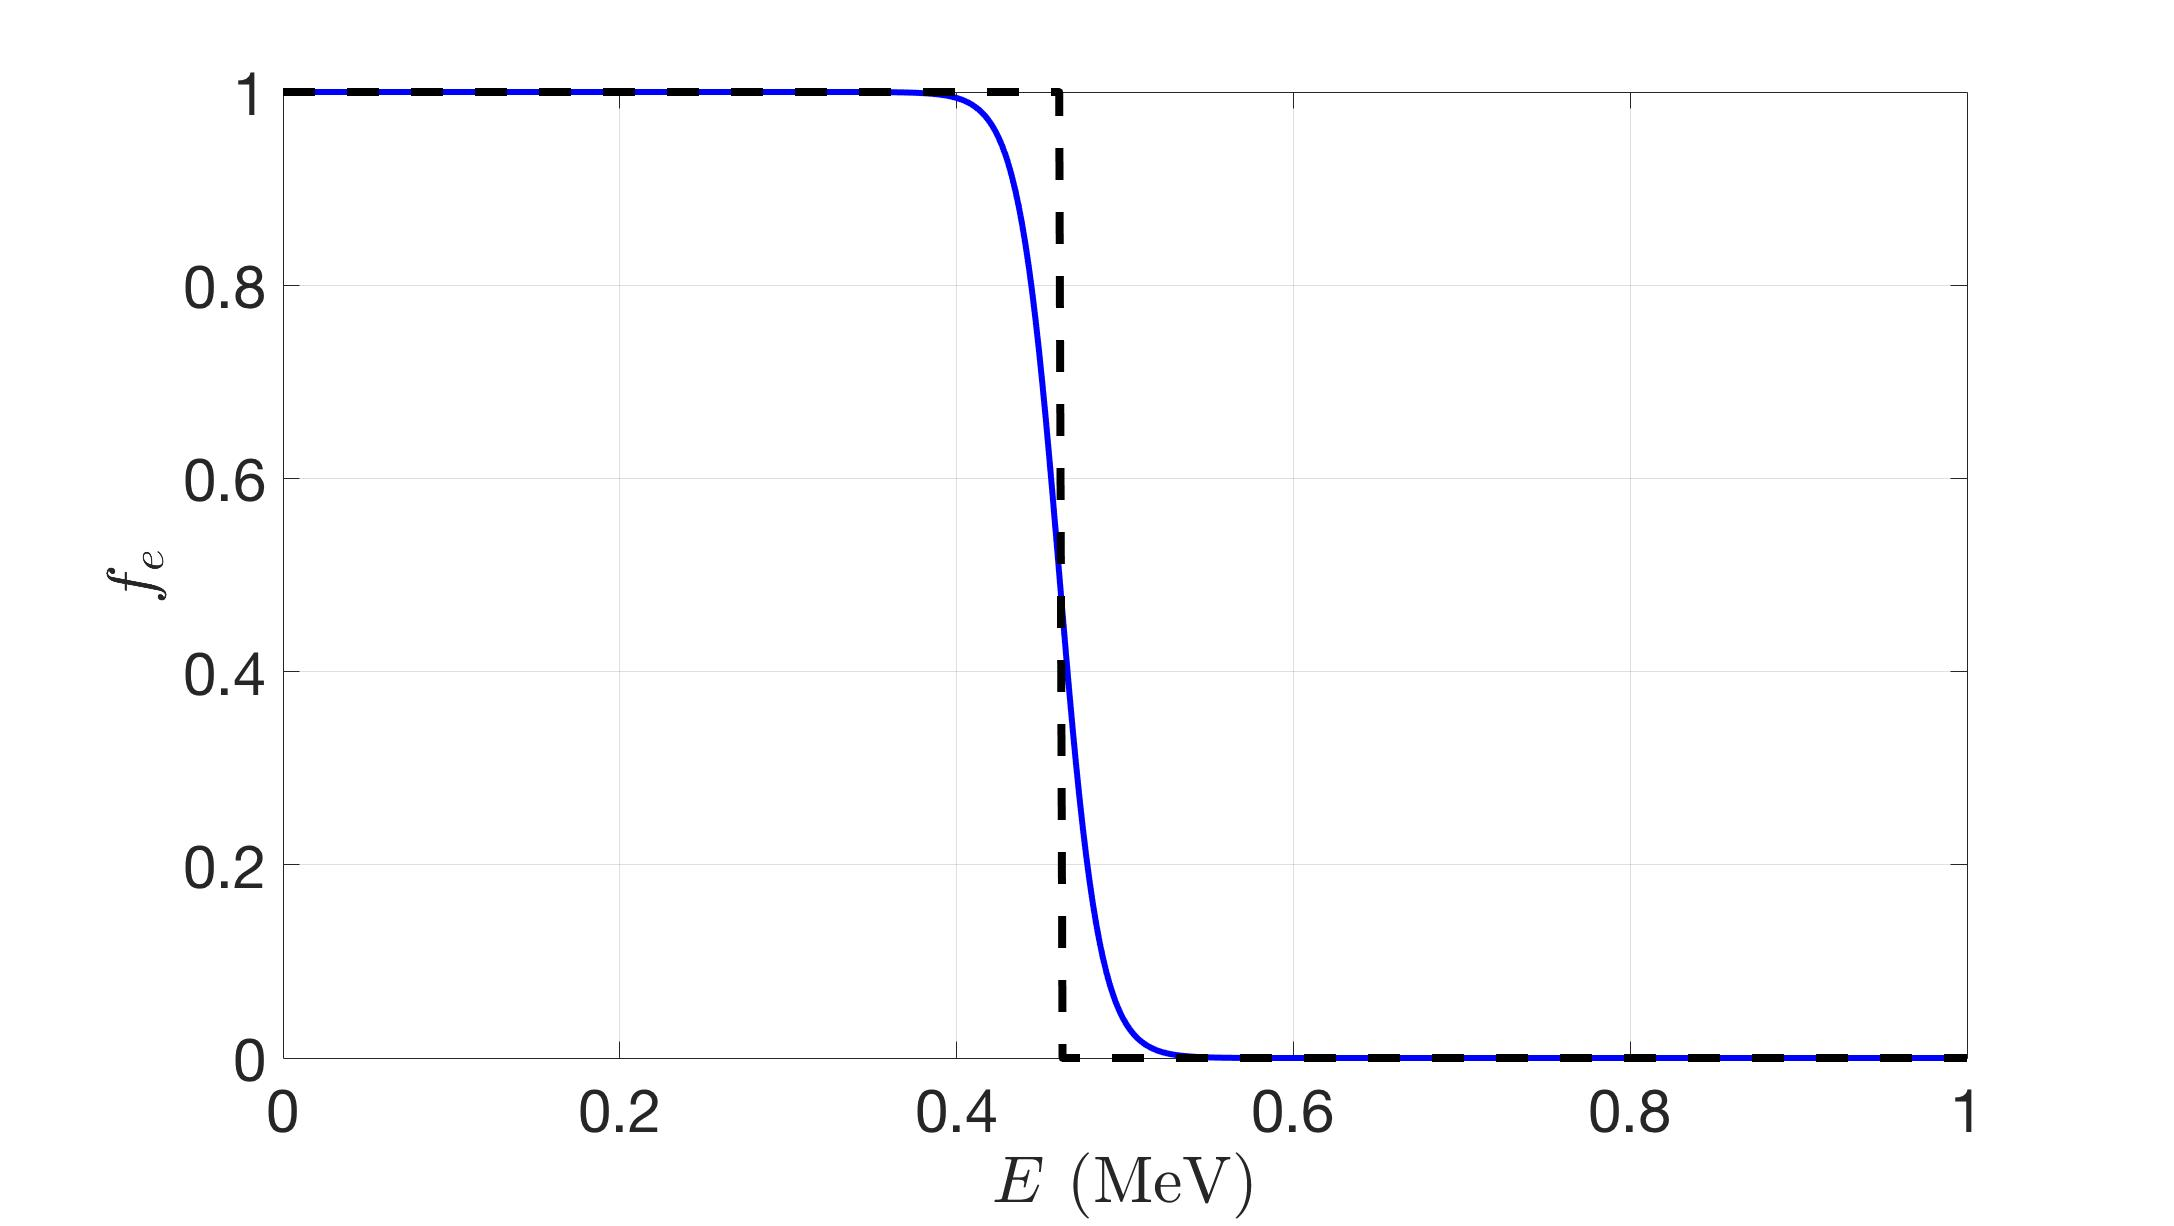
\includegraphics[width=0.9\textwidth]{./plot/Electron_distribution001}
\caption{The FD distribution is plotted (solid blue line) as a function of energy with parameters $T=0.012\MeV$ and $\widetilde\mu=0.461\MeV$. The zero temperature distribution is plotted as the dashed black line.}
\label{Electron_001}
\end{figure}
%%%%%%%%%%%%%%%%%%%%%%%%%%%%%%%%%%%%%%%

In \rf{Electron_001} we plot the FD distribution of a fermion as a function of energy with example parameters $T=0.012\MeV$ and $\widetilde\mu=0.461\MeV$. This shows the textbook behavior that for finite temperatures, there is a filling of some higher energy states above the chemical potential $\widetilde\mu$ at the expense of states below $\widetilde\mu$. As the temperature increases, the distribution becomes more broad as a wide range of states become thermally populated.

%%%%%%%%%%%%%%%%%%%%%%%%%%%%%%%%%%%%%%%
\section{Zero and finite temperature Fermi-Dirac distributions}
%\section{Exact finite temperature correction to Fermi distribution}
\label{NewFermi}
\subsection{A novel form of Fermi-Dirac distribution}
Our interest and motivations in studying the Fermi-Dirac distribution were to perform cosmological computations involving both high and low temperature physics. In doing so, we have identified the following novel way to write FD distribution as three terms which separates out the zero temperature portion from the finite temperature contributions as 
\begin{align}
\label{NFF1}
\begin{split}
f_\mathrm{FD}(x)
&=\left[e^{x}+1\right]^{-1}\\
&=\Theta(-x)+\frac{1}{2}e^{-|x|}\left[\sgn(x)+\tanh(x/2)\right]\,,\quad
x\equiv\frac{E-\widetilde\mu}{T}\,,
\end{split}
\end{align}
\begin{align}
\label{NFF2}
\Theta(x)=\left\{
\begin{array}{r}
1,\quad\mathrm{for}\quad{x}>0\\
1/2,\quad\mathrm{for}\quad{x}=0\\
0,\quad\mathrm{for}\quad{x}<0
\end{array}\right.\,,\qquad
\sgn(x)=\left\{
\begin{array}{r}
+1,\quad\mathrm{for}\quad{x}>0\\
0,\quad\mathrm{for}\quad{x}=0\\
-1,\quad\mathrm{for}\quad{x}<0\\
\end{array}\right.\,,
\end{align}
where $\Theta(x)$ is the Heaviside step function and $\sgn(x)$ is the sign function. The first term in \req{NFF1} represents the zero temperature portion of the FD distribution while the finite temperature terms are weighted by a decaying exponential function. The immediate benefit of this form is that numerical evaluations will naturally center around the Fermi surface of the system with finite temperature contributions exponentially weighted.

We note that the right hand side (RHS) of \req{NFF1} comprises of distributions rather than analytical functions~\cite{arfken_2011}. On first sight, it is difficult to see that these cancel to create the analytical FD function seen on the left hand side (LHS) of \req{NFF1}. In the following section, we will show that both sides are truly equivalent.

\subsection{Mathematical proof}
Considering the sign and step function properties given in \req{NFF2}, we see that \req{NFF1} is equal to $1/2$ when $x=0$. This is the expected behavior of the FD distribution when the energy is equal to the chemical potential. To further demonstrate that \req{NFF1} is indeed the FD distribution, we will use the following properties of the sign and step functions
\begin{align}
\label{NFF2a}
\sgn(x)\equiv\frac{|x|}{x}\equiv\frac{x}{|x|}\,,\quad
\sgn(x)=2\Theta(x)-1\,,\quad
\Theta(x)+\Theta(-x)=1\,.
\end{align}
We also write the following hyperbolic expression
\begin{equation}
\label{NFFa1}
\sgn^{2}(x)\sinh(x)=\sinh(x)\,.
\end{equation}
\req{NFFa1} is useful because while $\sgn^{2}(0)$ has an indeterminate value, $\sinh(0)=0$ vanishes; therefore we will not worry about this indeterminacy at the origin.

Using \req{NFF2a}, we replace the step function and exponential functions in \req{NFF1} with the following expressions
\begin{align}
\label{NFF4}
&\Theta(-x)=\frac 1 2 (1-\sgn(x))\,,\\ 
&e^{-|x|}=\cosh|x|-\sinh|x|=\cosh(x)- \sgn(x)\sinh(x)\,.
\end{align}
Therefore we can rewrite the FD distribution \req{NFF1} as
\begin{align}
\begin{split}
\label{NFF4a}
f_\mathrm{FD}(x)&=\frac{1}{2}\left[1-\sinh(x)+\cosh(x)\tanh(x/2)\right]\\
&+\frac{1}{2}\sgn(x)\left[\cosh(x)-1-\sinh(x)\tanh(x/2)\right]\,.
\end{split}
\end{align}
Using the properties of the hyperbolic functions
\begin{align}
\cosh(x)-1=2\sinh^2(x/2)\,,\qquad
\sinh(x)=2\sinh(x/2)\cosh(x/2)\,,
\end{align}
\req{NFF4a} then simplifies to
\begin{align}
\begin{split}
\label{NFF4b}
f_\mathrm{FD}(x)
&=\frac{1}{2}\left[1-\sinh(x)+\cosh(x)\tanh(x/2)\right]\,,\\
&=\frac{1}{2}\left[1-\tanh(x/2)\right]\,,\\
&=\left[e^{x}+1\right]^{-1}\,,
\end{split}
\end{align}
which is just the original FD distribution written in the usual manner \req{f_old}.

Lastly, we check that the properties of the first derivative of \req{NFF1} are in agreement with the usual FD distribution. We write the first derivative of the singular distributions as 
\begin{align}
\label{NFF1b}
\frac{d}{dx}\Theta(-x)&=-\delta(x)\,,\qquad 
\frac{d}{dE}\Theta(-x)=-\frac{1}{T}\delta(x)\,,\\
\frac{d}{dx}\sgn(x)&={\color{red}2\delta(x)}\,,\,\,\quad 
\frac{d}{dE}\sgn(x)={\color{red}\frac{2}{T}\delta(x)}\,,
\end{align}
both without and with units and where $\delta(x)$ is the Dirac $\delta$-function. These cancel in \req{NFF1} {\color{red} at $x=0$} exactly as required since the derivative of the FD distribution written in \req{f_old} lacks a $\delta$-function. This encourages us to believe that all of singular expressions cancel leaving it fully analytic. This completes our demonstration of the validity of \req{NFF1}. 

\subsection{Numerical illustration}
In Fig.~\ref{Fermi_Checking} we plot the exact Fermi-distribution (LHS of Eq.~(\ref{NFF1}) with solid lines and novel form of Fermi-distribution (RHS of Eq.~(\ref{NFF1})) with dashed lines as a function of energy with different parameters. It demonstrate that 
LHS and RHS of Eq.~(\ref{NFF1}) are equivalent to each other numerically.

%~~~~~~~Figure~~~~~~~~~~~~~~~~~~~~~~~~~~~~~~~~~~~~~~~~~~~~~~~~~~~~~~~~~~~~~~~~~~~~~~~~~~~~~~~~~~~~~
\begin{figure}[ht]
\begin{center}
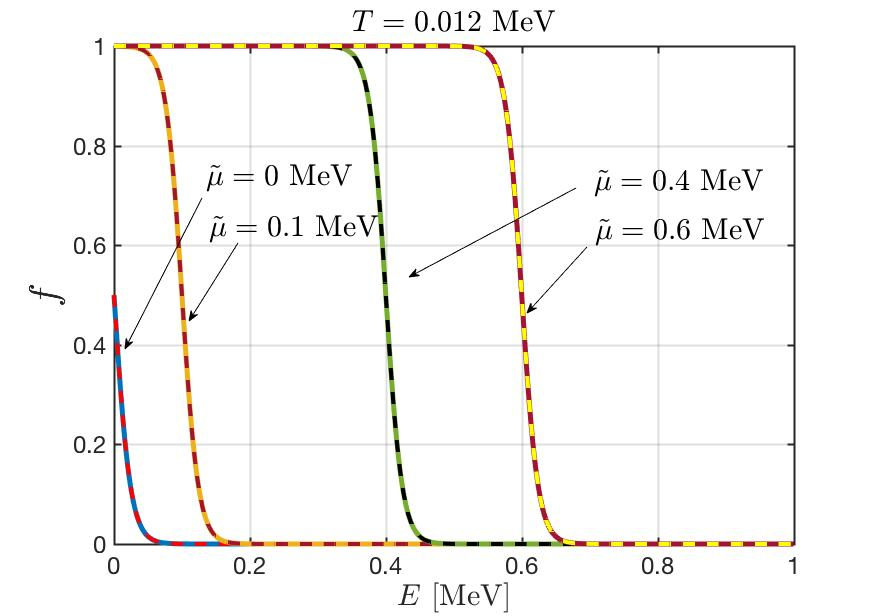
\includegraphics[width=0.5\textwidth]{./plot/Fermi_novel_001}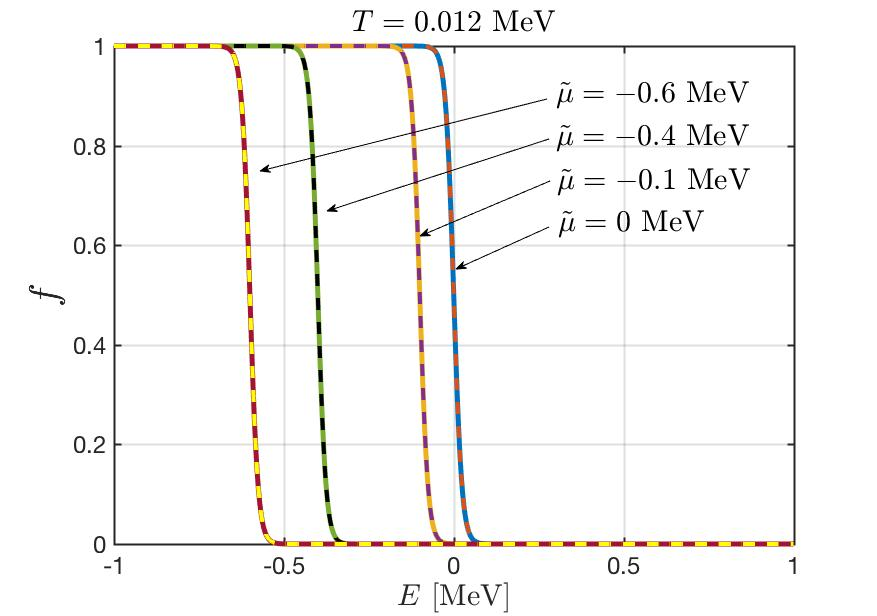
\includegraphics[width=0.5\textwidth]{./plot/Fermi_novel_002}
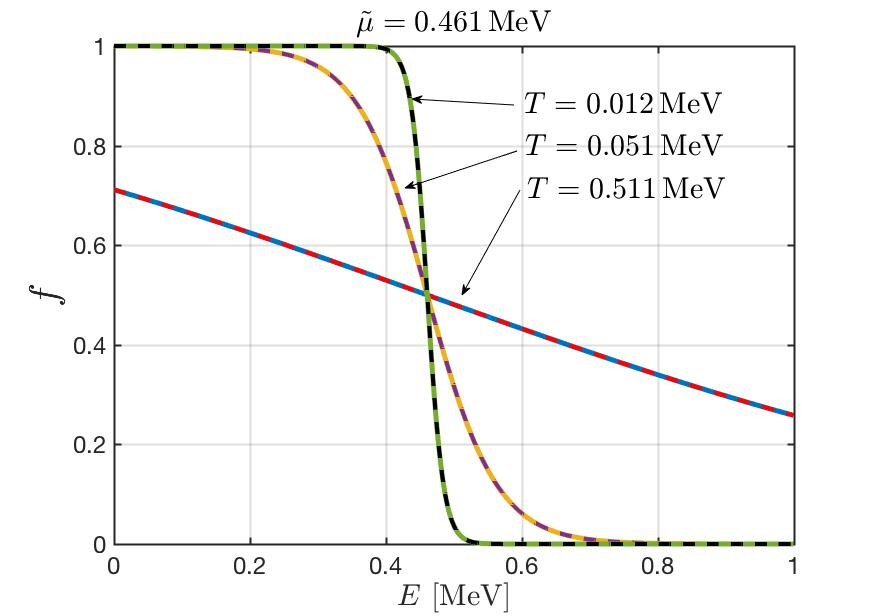
\includegraphics[width=0.5\textwidth]{./plot/Fermi_novel_003}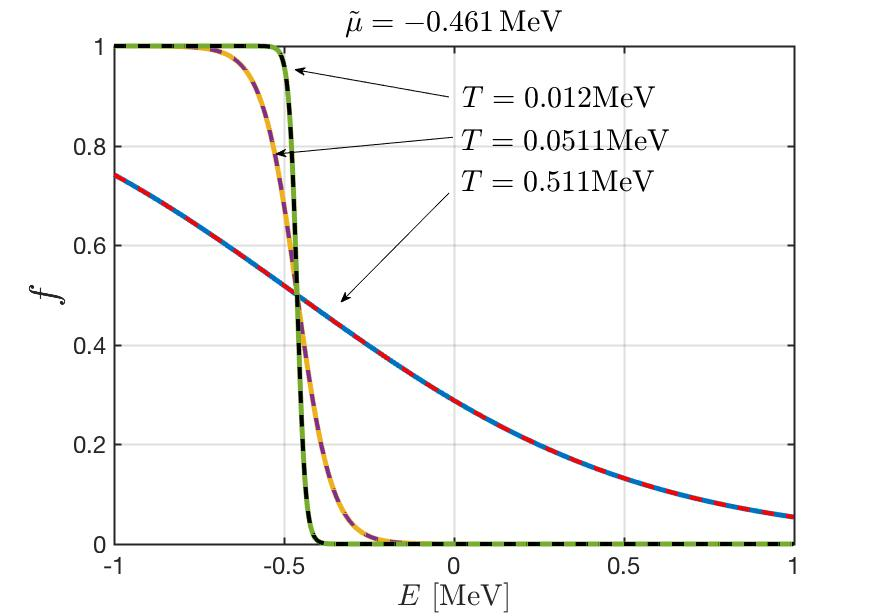
\includegraphics[width=0.5\textwidth]{./plot/Fermi_novel_004}
\caption{The exact Fermi-distribution (LHS of Eq.~(\ref{NFF1}) with solid lines and novel form of Fermi-distribution (RHS of Eq.~(\ref{NFF1})) with dashed lines as a function of energy with different parameters.Top: we compare the RHS and LHS of Eq.~(\ref{NFF1}) with different chemical potential: $\widetilde\mu=0, \pm0.1, \pm0.4\,\pm0.6\, \mathrm{MeV}$ at temperature $T=0.012\,\mathrm{MeV}$. Bottom: the Fermi distribution with different temperatures $T=0.511, 0.0511, 0.012\,\mathrm{MeV}$ for chemical potential $\widetilde\mu=\pm0.461\,\mathrm{MeV}$.}
\label{Fermi_Checking}
\end{center}
\end{figure}
%~~~~~~~~~~~~~~~~~~~~~~~~~~~~~~~~~~~~~~~~~~~~~~~~~~~~~~~~~~~~~~


%%%%%%%%%%%%%%%%%%%%%%%%%%%%%%%%%%%%%%%%%%%%%%%%%%%%%%%%%%%%%%%%%%%%%%%%%

\section{Partition function and Magnetization}\label{NumericalResult}

In previous section we demonstrate that the Fermi-distribution can be written into a novel form Eq.~(\ref{NFF1}). To illustrate the benefits of our innovative Fermi distribution function in practical applications, it is convenient to introduce the partition function and consider the physical quantity magnetization as a example.

Considering the partition function of $e^\pm$ gas in a uniform magnetic field $B$ pointing along the $z$-axis, we have
\begin{align}
\ln\mathcal{Z}_{tot}=eBV\!\!\sum_{s=\pm1}\sum_{j=0}^\infty\int^\infty_{-\infty} \!\!dp_z\bigg[\ln\left(1+e^{-\beta(E_{j,s}-\mu_e)}\right)+\ln\left(1+e^{-\beta(E_{j,s}+\mu_e)}\right)\bigg],
\end{align}
where $\beta=1/T$, $\mu_e$ is the chemical potential of electron, and the electron(positron) energy $E_{j,s}$ can be written as
\begin{align}
E_{j,s}&=\sqrt{m^2_e+p^2_z+2eB\left(j+\frac{1}{2}+\frac{g}{4}s\right)},\qquad s=\pm1,\qquad j=0,1,2,\dots
\end{align}
To simplify the integral over $dp_z$ we can take  the integration by integrating by part and obtain
\begin{align}
&\int^\infty_{-\infty} \!\!dp_z\bigg[\ln\left(1+e^{-\beta(E_{j,s}-\mu_e)}\right)+\ln\left(1+e^{-\beta(E_{j,s}+\mu_e)}\right)\bigg]\notag\\
&=2\bigg[\int_0^\infty\!\!dp_z\ln\left(1+e^{-\beta(E_{j,s}-\mu_e)}\right)+\int_0^\infty\!\!dp_z\ln\left(1+e^{-\beta(E_{j,s}+\mu_e)}\right)\bigg]\\
&=2\bigg[\beta\int_0^\infty\!\!dp_z p_z\frac{\partial E_{j,s}}{\partial p_z}\frac{1}{e^{\beta(E_{j,s}-\mu_e})+1}+\beta\int_0^z\!\!dp_z p_z\frac{\partial E_{j,s}}{\partial p_z}\frac{1}{e^{\beta(E_{j,s}+\mu_e})+1}\bigg]\\
&=2\beta\int_0^\infty\!\!dp_z \frac{p_z^2}{E_{j,s}}\left[\frac{1}{e^{\beta(E_{j,s}-\mu_e})+1}+\frac{1}{e^{\beta(E_{j,s}+\mu_e})+1}\right]
\end{align}

Then the partition function of $e^\pm$ plasma in a uniform magnetic field $B$ can be written as
\begin{align}
\ln\mathcal{Z}_{tot}&=eBV\sum_{s=\pm1}\sum_{j=0}^\infty2\beta\int_0^\infty\!\!dp_z \frac{p_z^2}{E_{j,s}}\left[\frac{1}{e^{\beta(E_{j,s}-\mu_e})+1}+\frac{1}{e^{\beta(E_{j,s}+\mu_e})+1}\right]\\
&=eBV\sum_{s=\pm1}\sum_{j=0}^\infty2\beta\int_0^\infty\!\!dp_z \frac{p_z^2}{E_{j,s}}\bigg[f_{e^-}+f_{e^+}\bigg].
\end{align}
Considering the case $g=2$, then we have
\begin{align}
&E_{j,+}=\sqrt{{m}_e^2+p^2_z+2eB\left(j+1\right)}\longrightarrow E_{n}=\sqrt{{m}_e^2+p^2_z+2eBn},\quad n=1,2,3,\dots\\
&E_{j,-}=\sqrt{{m}_e^2+p^2_z+2eB\left(j\right)}\longrightarrow E_{n}=\sqrt{{m}_e^2+p^2_z+2eBn},\,\, n=0,1,2,3,\dots
\end{align}
where we change the index from $j$ to $n$. In this case, the partition function of $e^\pm$ plasma can be written as
\begin{align}
\ln\mathcal{Z}_{tot}&=V(2eB\beta) \bigg[ \sum_{n=1}^\infty\int_0^\infty\!\!dp_z \frac{p_z^2}{E_{n}}\bigg(f_{e^-}(E_n)+f_{e^+}(E_n)\bigg)+\sum_{n=0}^\infty\int_0^\infty\!\!dp_z \frac{p_z^2}{E_{n}}\bigg(f_{e^-}(E_n)+f_{e^+}(E_n)\bigg)\bigg]\notag\\
&=V(2eB\beta) \bigg[\int_0^\infty\!\!dp_z \frac{p_z^2}{E_0}\bigg(f_{e^-}(E_0)+f_{e^+}(E_0)\bigg)+2 \sum_{n=1}^\infty\int_0^\infty\!\!dp_z \frac{p_z^2}{E_{n}}\bigg(f_{e^-}(E_n)+f_{e^+}(E_n)\bigg)\bigg]\notag\\
&=V(2eB\beta)\bigg(\ln\mathcal{I}_{0}+\ln\mathcal{I}_{n}\bigg)
\end{align}
where the ground energy is given by $E_0=\sqrt{{m}_e^2+p^2_z}$ and the partition function $\ln\mathcal{I}_{0}$ and $\ln\mathcal{I}_{n}$ are defined as
\begin{align}
&\ln\mathcal{I}_{0}=\int_0^\infty\!\!dp_z \frac{p_z^2}{E_0}\bigg(f_{e^-}(E_0)+f_{e^+}(E_0)\bigg),\qquad E_0=\sqrt{{m}_e^2+p^2_z} \\
&\ln\mathcal{I}_{n}=2 \sum_{n=1}^\infty\int_0^\infty\!\!dp_z \frac{p_z^2}{E_{n}}\bigg(f_{e^-}(E_n)+f_{e^+}(E_n)\bigg),\quad E_n=\sqrt{{m}_e^2+p^2_z+2eBn}
\end{align}

Giving the partition function, the magnetization can be obtained via the definition
\begin{align}
M&=\frac{1}{V\beta}\frac{\partial \ln \mathcal{Z}_{tot}}{\partial B}=2e\frac{\partial}{\partial B}\bigg[B\bigg(\ln\mathcal{I}_{0}+\ln\mathcal{I}_{n}\bigg)\bigg]=M_0+M_n,\\
&M_0=2e\ln\mathcal{I}_{0},\qquad
\label{M_landau}
M_n=2e\bigg(\ln\mathcal{I}_{n}+B\frac{\partial\ln\mathcal{I}_n}{\partial B}\bigg)
\end{align}
where we introduce the magnetization $M_0$ and $M_n$ to simplify the notations. 
Integrating by part the magnetization $M_n$ can be written as
\begin{align}
M_n&=4e\sum_{n=1}^\infty \int_{m_n}^\infty\!\!dE_n\bigg(f_{e^-}(E_n)+f_{e^+}(E_n)\bigg)\left[{\sqrt{E^2_n-m^2_n}}-\frac{Ben}{\sqrt{E^2_n-m^2_n}}\right]\\
&=4e\sum_{n=1}^\infty \int_{0}^\infty\!\!dp_z\frac{p_z}{E_n}\bigg(f_{e^-}(E_n)+f_{e^+}(E_n)\bigg)\left[\frac{p_z^2-Ben}{p_z}\right]\\
&=4e\sum_{n=1}^\infty \int_{0}^\infty\!\!dp_z\frac{(p_z^2-Ben)}{E_n}\bigg(f_{e^-}(E_n)+f_{e^+}(E_n)\bigg)\\
&=4e \int_{0}^\infty\!\!dp_z\sum_{n=1}^\infty\frac{(p_z^2-Ben)}{E_n}\bigg(f_{e^-}(E_n)+f_{e^+}(E_n)\bigg).
\end{align}


It is convenient to introduce the dimensionless variables and critical magnetic field $B_c$ as follows:
\begin{align}
\xi=p_z/T,\qquad \eta=m_e/T,\qquad B_c=m^2_e/e
\end{align}
In this case, the magnetization $M_0$ and $M_n$ can be written as
\begin{align}
&M_0=2eT^2\int_0^\infty\!\!d\xi\, F_0(E_0/T),\qquad M_n=2eT^2\int_{0}^\infty\!\!d\xi\left(2\sum_{n=1}^\infty\,F_n(E_n/T)\right)
\end{align}
where the $M_0$ represents the background magnetization  and $M_n$ is magnetization associate to Landau level. The function $F_n$ is defined as
\begin{align}
&F_n=\frac{(\xi^2-\eta^2nB/B_c)}{\sqrt{\xi^2+\eta^2\left(1+2nB/B_c\right)}}\bigg(f_{e^-}(E_n/T)+f_{e^+}(E_n/T)\bigg)\\
&E_n/T=\sqrt{\xi^2+\eta^2\left(1+2nB/B_c\right)},\qquad n=0,1,2,\cdots
\end{align}

To illustrate the benefits of our novel Fermi distribution function in calculation of magnetization, it is convenient to rewrite the Fermi-function as 
\begin{align}
&f=f_{\mathrm{T=0}}+f_\mathrm{T\neq0}+\tilde f_\mathrm{T\neq0}
\end{align}
where the functions $f_{\mathrm{T=0}}$, $f_\mathrm{T\neq0}$ ans $\tilde f_\mathrm{T\neq0}$ are defined as
\begin{align}
&f_{\mathrm{T=0}}=\Theta(\widetilde\mu-E),\\
&f_\mathrm{T\neq0}=\frac{1}{2}\,e^{-|E-\widetilde\mu|/T}\frac{(E-\widetilde\mu)}{|E-\widetilde\mu|},\\ 
&\tilde f_\mathrm{T\neq0}=\frac{1}{2}\,e^{-|E-\widetilde\mu|/T}\tanh\bigg(\frac{E-\widetilde\mu}{2T}\bigg),
\end{align}
In this case, the function $F_n$ can be written as
\begin{align}
&F_n=F_n^{\mathrm{T=0}}+F_n^{\mathrm{T\neq0}}+\widetilde F_n^{\mathrm{T\neq0}},\\
&F_n^{\mathrm{T=0}}=\frac{(\xi^2-\eta^2nB/B_c)}{\sqrt{\xi^2+\eta^2\left(1+2nB/B_c\right)}}\bigg(f^{\mathrm{T=0}}_{e^-}(E_n/T)+f^{\mathrm{T=0}}_{e^+}(E_n/T)\bigg)\\
&F_n^{\mathrm{T\neq0}}=\frac{(\xi^2-\eta^2nB/B_c)}{\sqrt{\xi^2+\eta^2\left(1+2nB/B_c\right)}}\bigg(f^{\mathrm{T\neq0}}_{e^-}(E_n/T)+f^{\mathrm{T\neq0}}_{e^+}(E_n/T)\bigg)\\
&\widetilde F_n^{\mathrm{T\neq0}}=\frac{(\xi^2-\eta^2nB/B_c)}{\sqrt{\xi^2+\eta^2\left(1+2nB/B_c\right)}}\bigg(\tilde f^{\mathrm{T\ne0}}_{e^-}(E_n/T)+\tilde f^{\mathrm{T\neq0}}_{e^+}(E_n/T)\bigg)
\end{align}
In Fig~\ref{F0_Checking}, we plot the background  $F_0$ as a function of $p_z/T$ with temperature $T=0.012$ MeV and chemical potential $\mu=2$ MeV. The dominant term is the $F_{n=0}^{\mathrm{T=0}}$ which correspond to the step function contribution when $T=0$ The functions $F_{n=0}^{\mathrm{T\neq0}}$ and $\widetilde F_{n=0}^{\mathrm{T\neq0}}$ provide the correction near the energy surface $\mu/T\approx166.6$ MeV.
%~~~~~~~~~~~~~~~~~~~~~~~~~~~~~~~~~~~~~~~~~~~~~~
\begin{figure}[ht]
\begin{center}
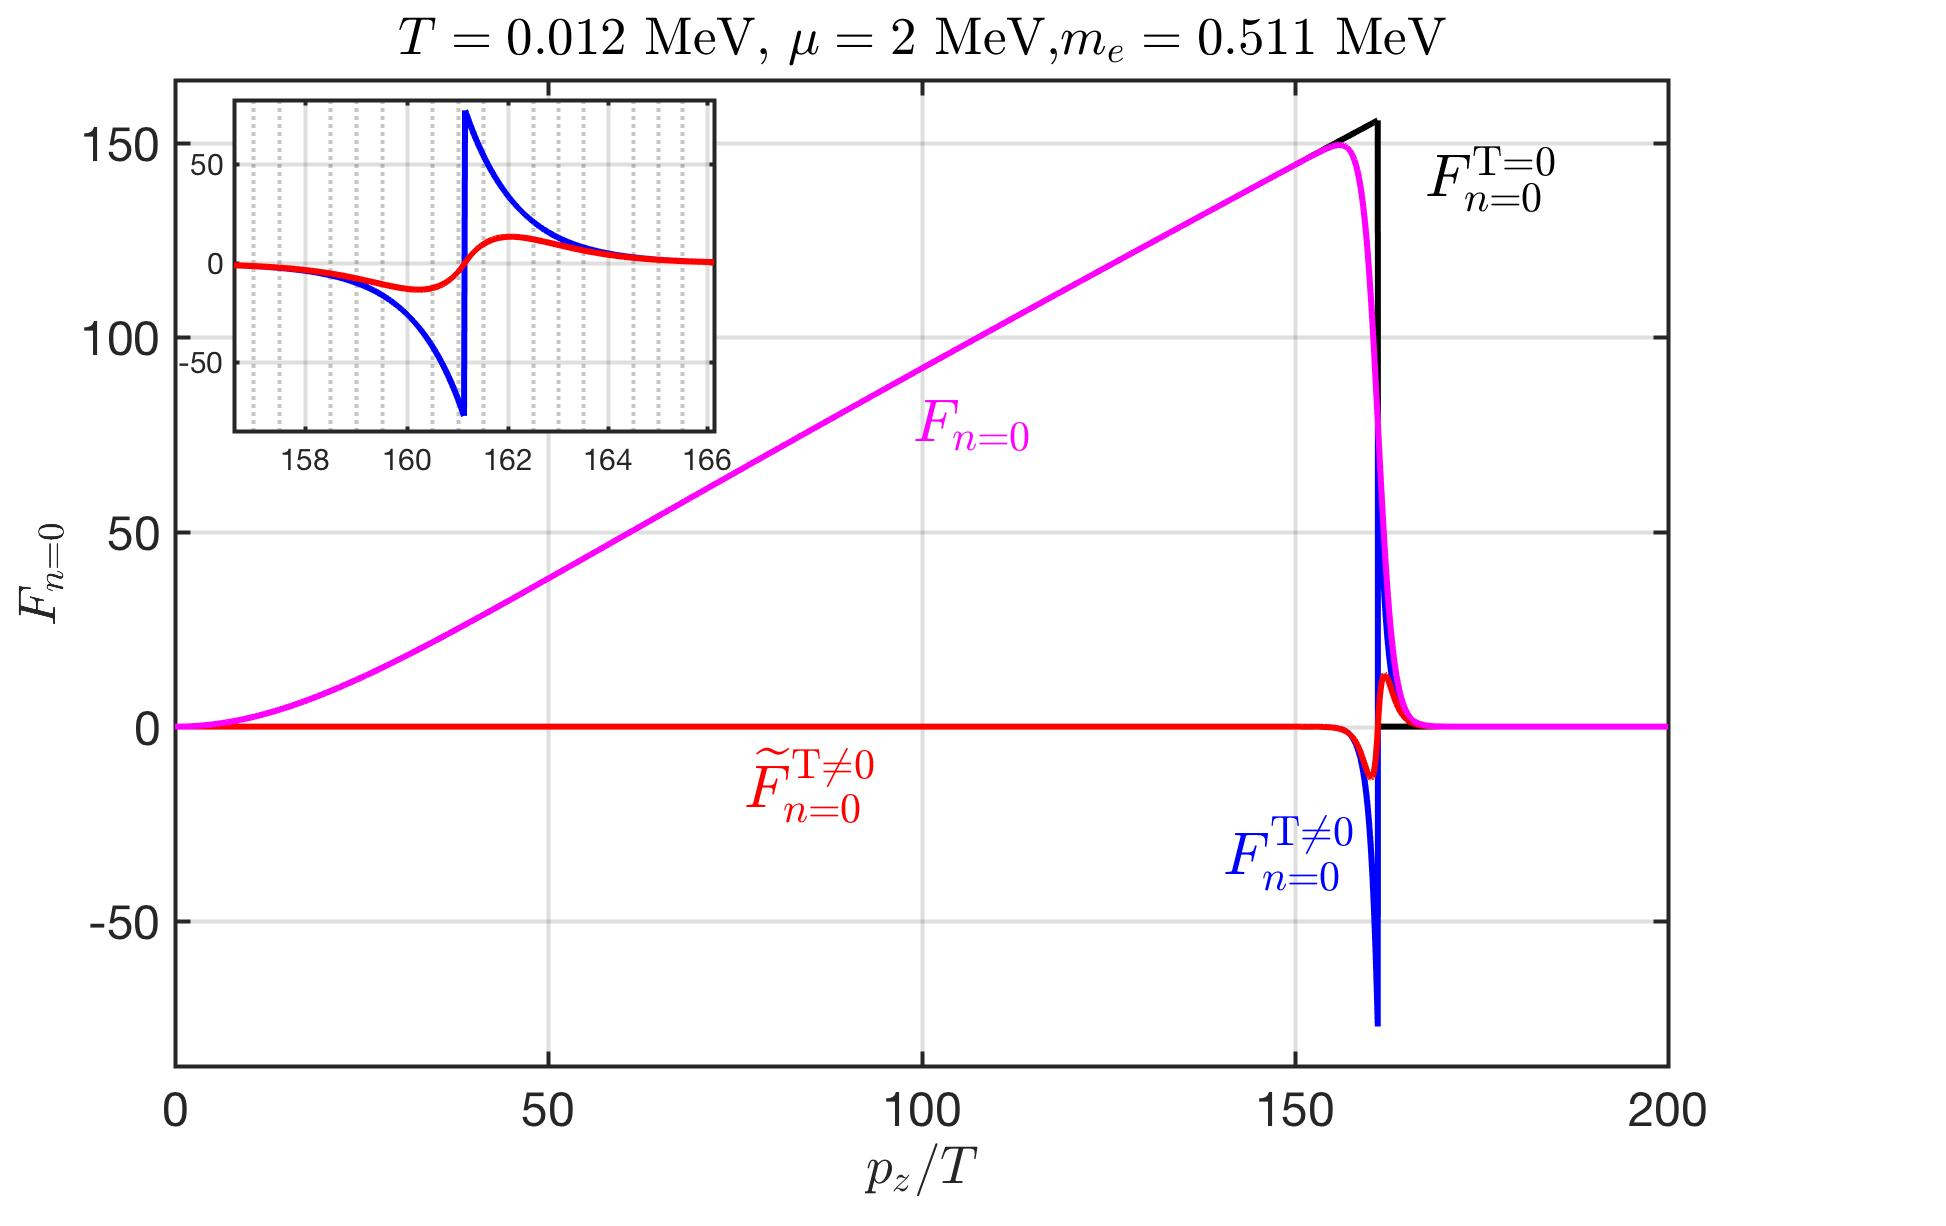
\includegraphics[width=0.9\textwidth]{./plot/NewFermi_Background}
%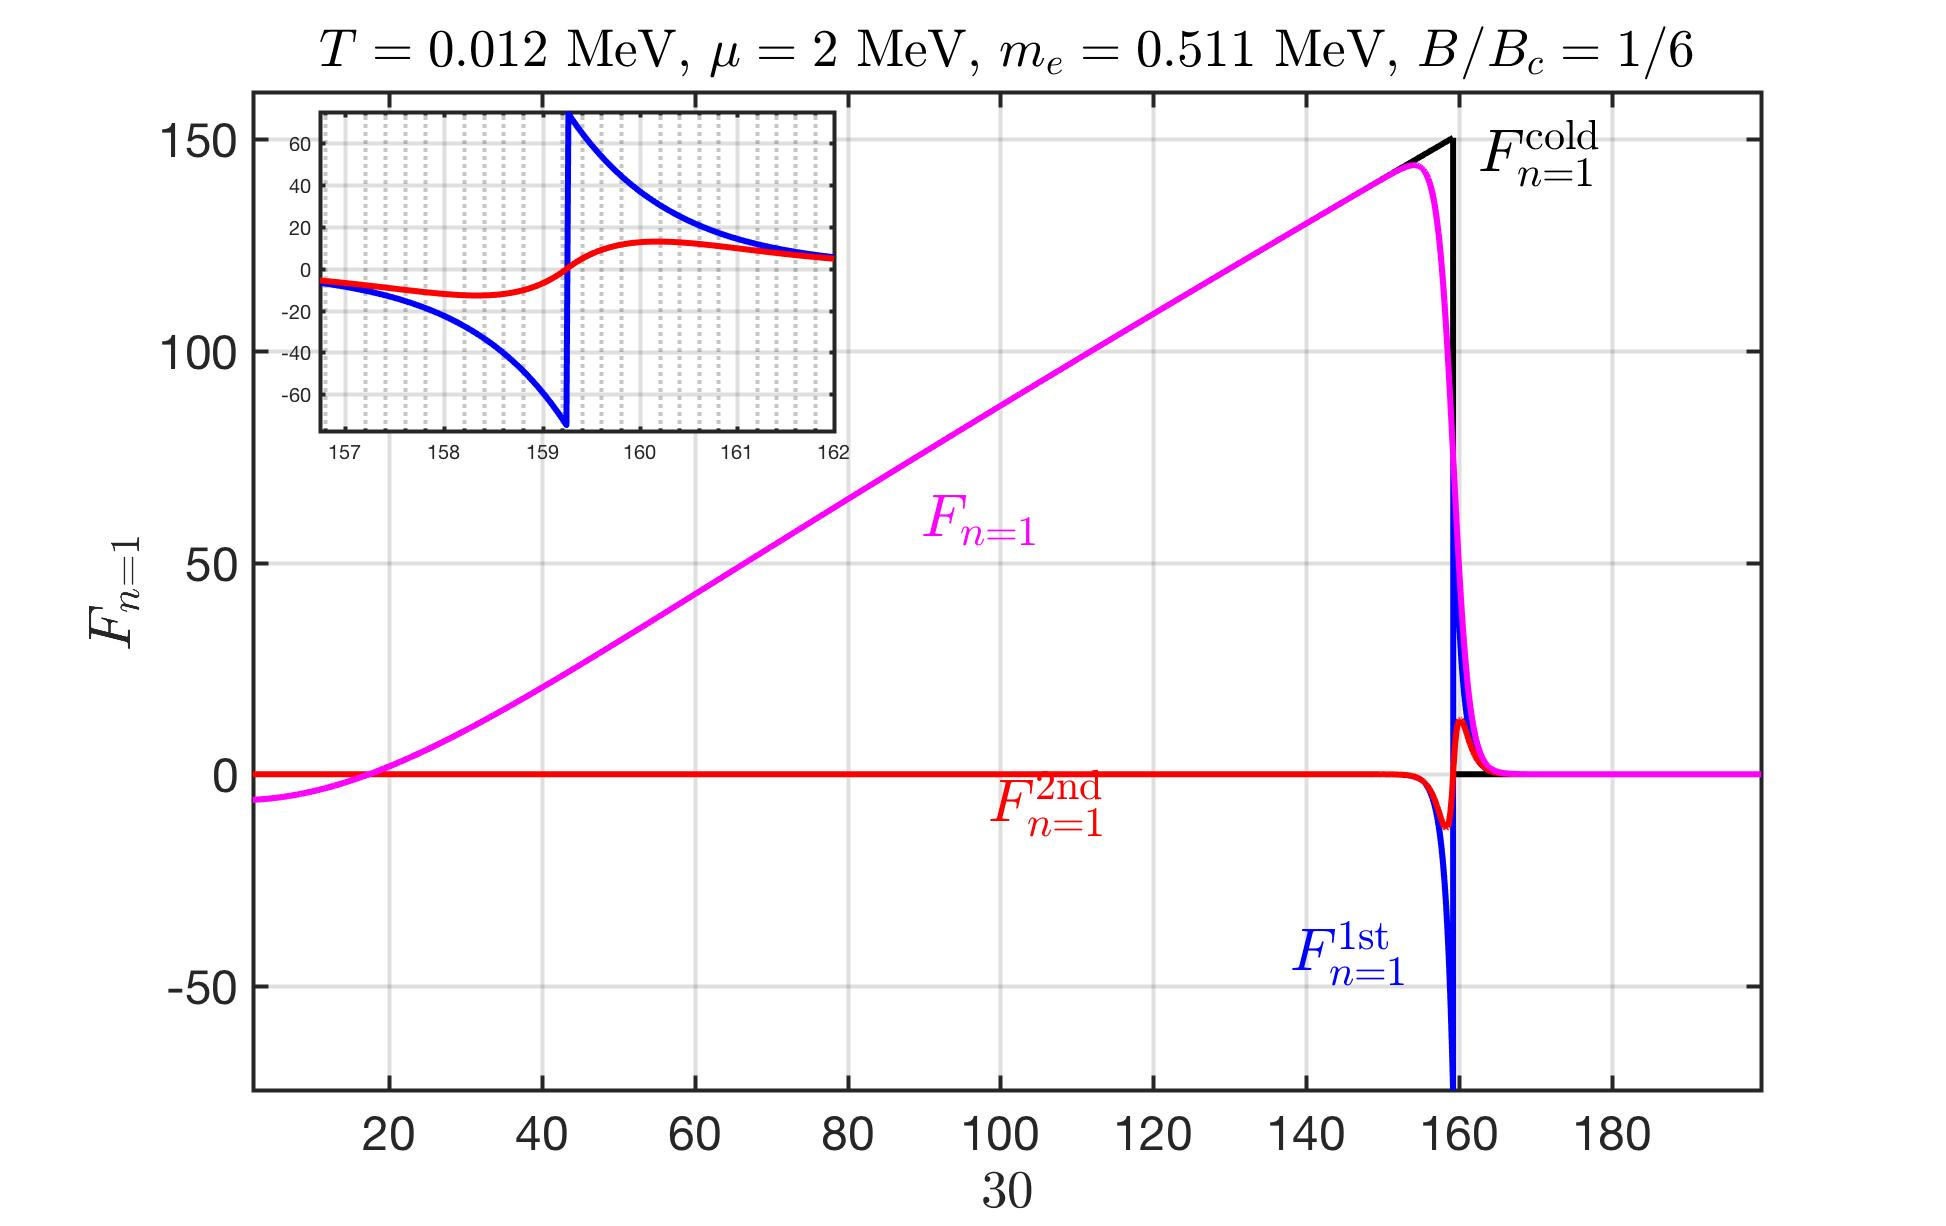
\includegraphics[width=0.9\textwidth]{./plot/NewFermi_Magnetization_n001}
\caption{The function $F_n$ as a function of $p_z/T$ for $n=0$ (purple line). We consider the case: $T=0.012$ MeV and $\mu=2$ MeV. For comparison, the black line represents $F_{n=0}^{\mathrm{T=0}}$, the blue line label $F_{n=0}^{\mathrm{T\neq0}}$ and red line is $\tilde F_{n=0}^{\mathrm{T\neq0}}$.}
\label{F0_Checking}
\end{center}
\end{figure}
%~~~~~~~~~~~~~~~~~~~~~~~~~~~~~~~~~~~~~~~~~~~~~~~~~~~


In Fig.~\ref{Fn_Checking} we plot the sum over $F_n$ as a function of $p_z/T$ with condition $T=0.012$ MeV, $\mu=2$ MeV and magnetic field $B/B_c=1/6$. It shows that for the given conditions, our novel form of Fermi function converge very fast. When $N=50$ the sum over Landau level is already stable.
%~~~~~~~~~~~~~~~~~~~~~~~~~~~~~~~~~~~~~~~~~~~~~~
\begin{figure}[ht]
\begin{center}
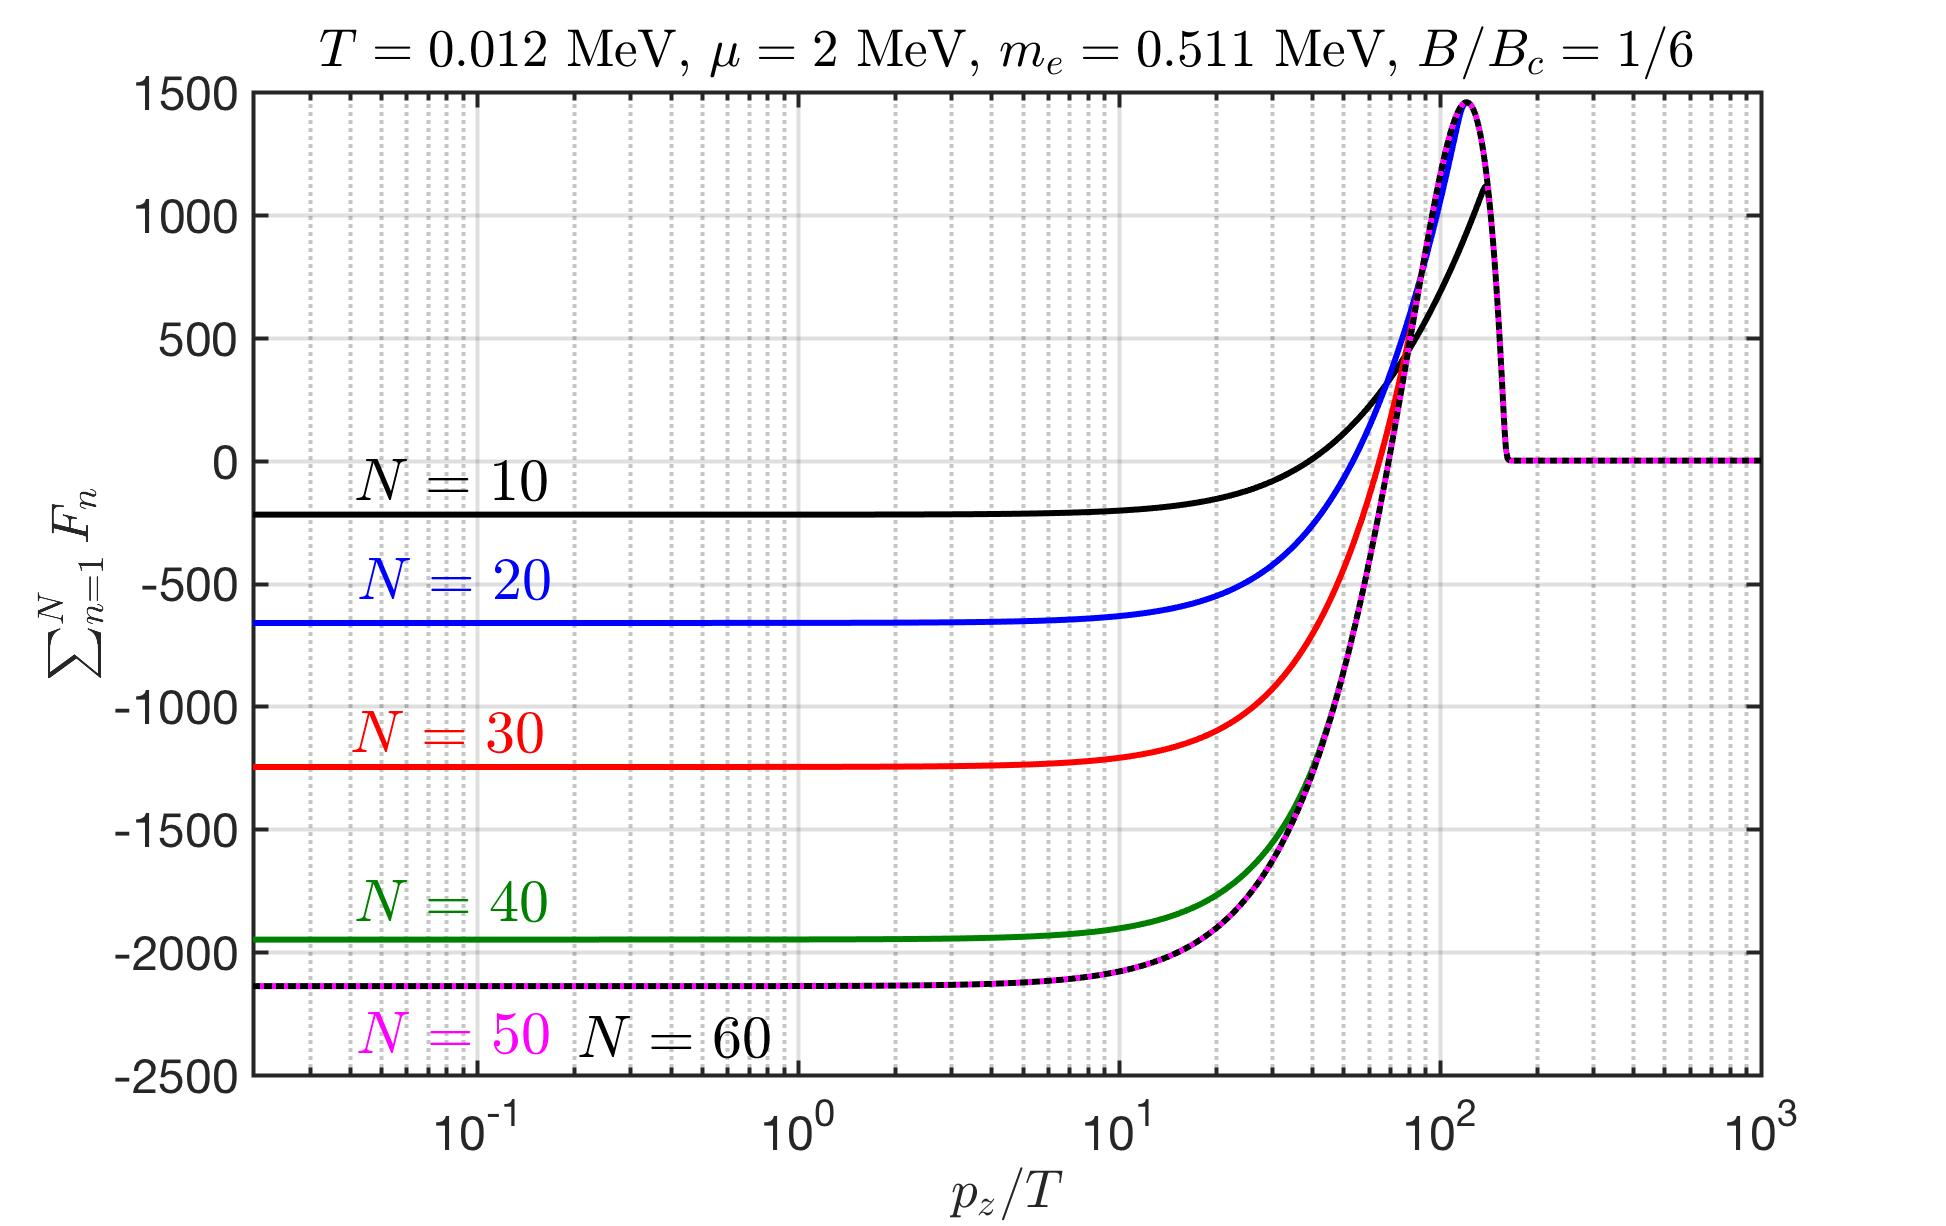
\includegraphics[width=0.9\textwidth]{./plot/NewFermi_SumChecking}
\caption{The sum over  $\sum_{n=1}^NF_n$ as a function of $p_z/T$ for different values of $N$. We consider the case: $T=0.012$ MeV, $\mu=2$ MeV and magnetic field $B/B_c=1/6$.}
\label{Fn_Checking}
\end{center}
\end{figure}
%~~~~~~~~~~~~~~~~~~~~~~~~~~~~~~~~~~~~~~~~~~~~~~~~~~~
%~~~~~~~~~~~~~~~~~~~~~~~~~~~~~~~~~~~~~~~~~~~~~~
\begin{figure}[ht]
\begin{center}
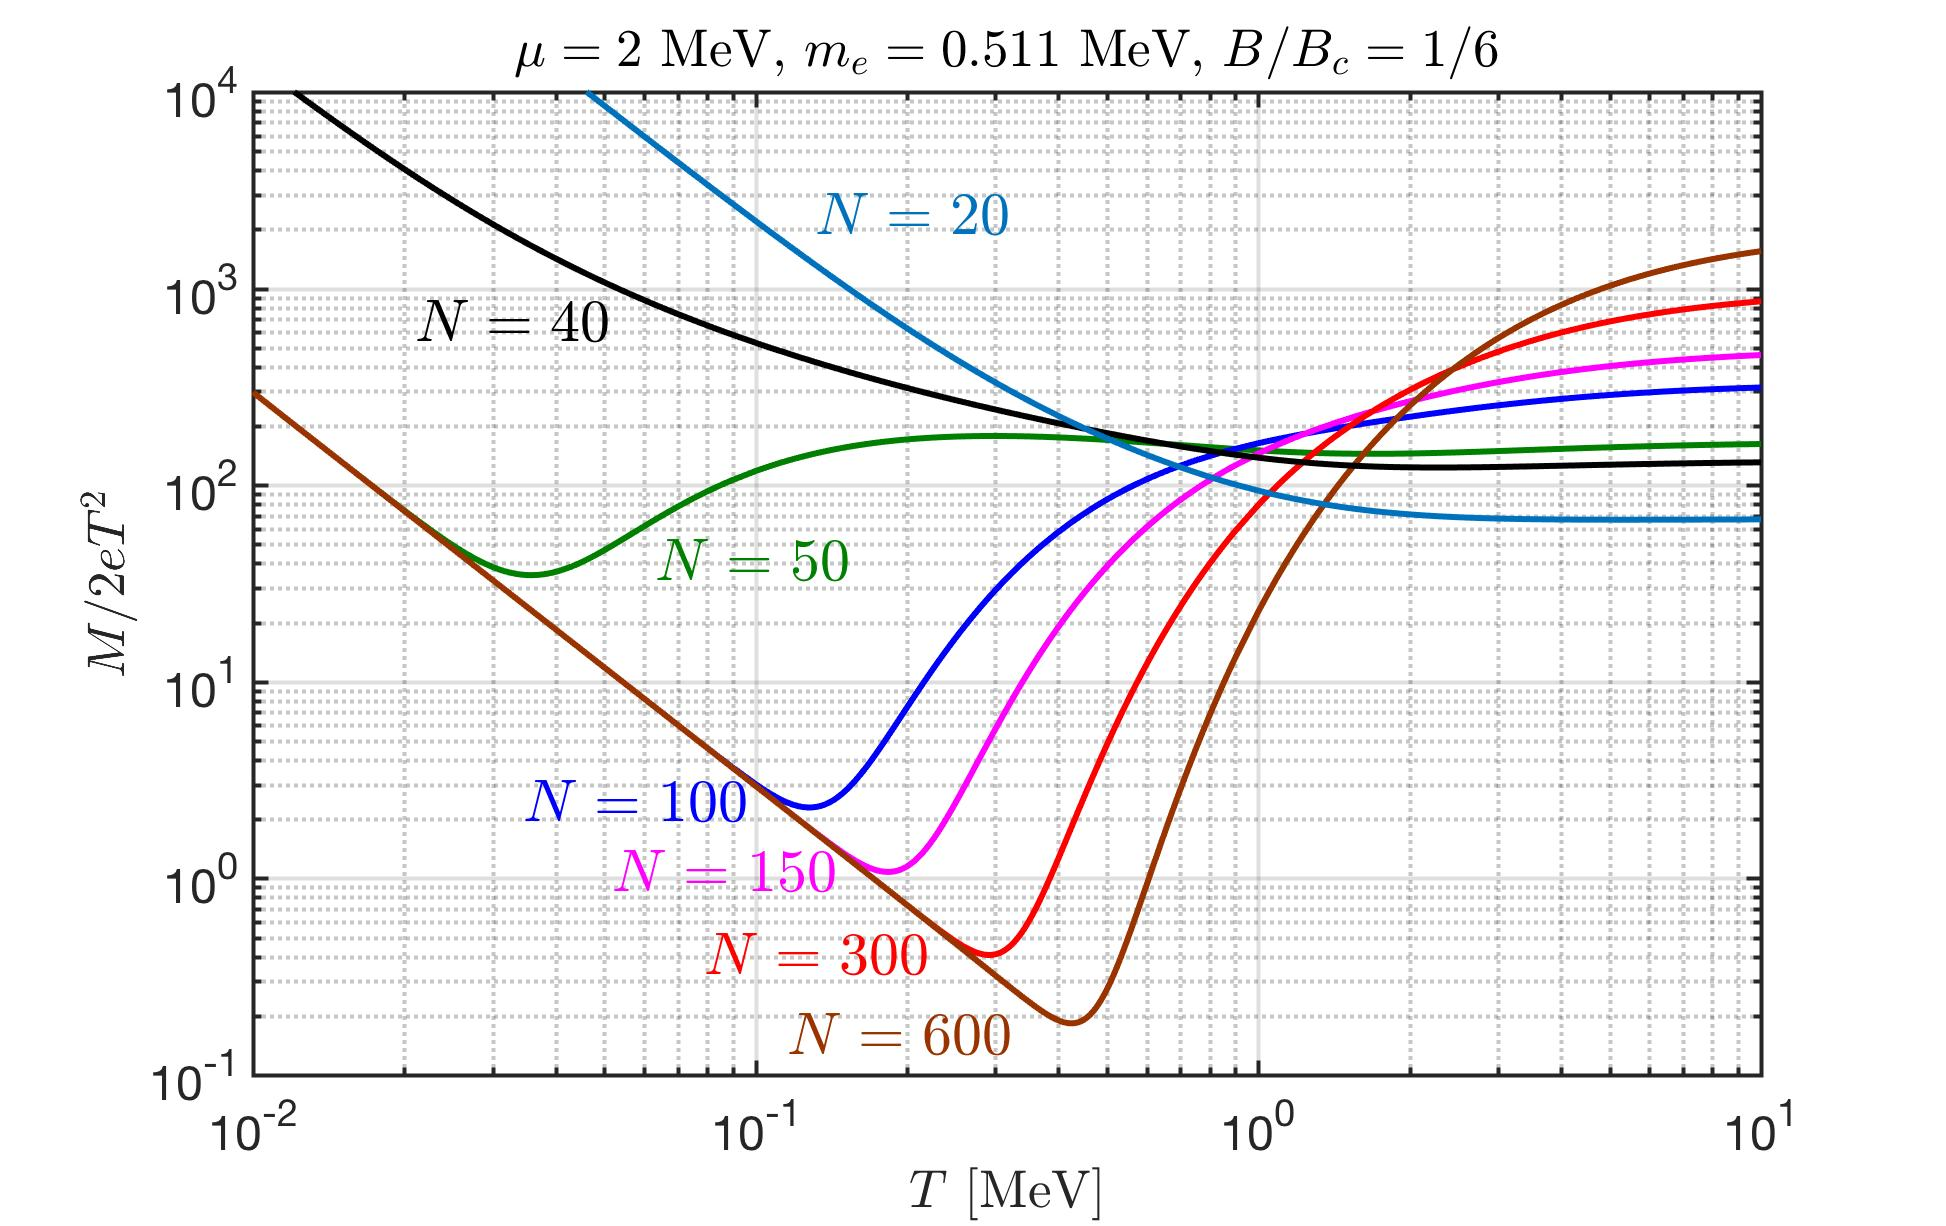
\includegraphics[width=0.9\textwidth]{./plot/NewFermi_Magnetization_tot003}
\caption{We plot the magnetization $M/2eT^2$ as a function of temperature with the conditions $\mu=2$ MeV and $B/B_c=1/6$}
\label{M_Checking}
\end{center}
\end{figure}
%~~~~~~~~~~~~~~~~~~~~~~~~~~~~~~~~~~~~~~~~~~~~~~~~~~~

In Fig.~\ref{M_Checking} we plot the magnetization $M/2eT^2$ as a function of temperature with the conditions $\mu=2$ MeV and $B/B_c=1/6$. It shows that the novel form of Fermi distribution can improve the numerical calculation of Landau level by summing over finite terms only. For different higher temperature range, instead of sum over a large numbers of $N$, we just need to include more terms in Landau level summation to obtain the stabilize magnetization.


\section{Results and Discussion}
\label{sec12}


\section{Appendix}
Considering the second term in magnetization $M_n$ Eq.~(\ref{M_landau}), it can be written as
\begin{align}
B\frac{\partial\ln\mathcal{I}_n}{\partial B}&=2B \sum_{n=1}^\infty\int_0^\infty\!\!dp_z \frac{\partial E_n}{\partial B}\frac{\partial}{\partial E_n}\left[\frac{p_z^2}{E_{n}}\bigg(f_{e^-}(E_n)+f_{e^+}(E_n)\bigg)\right]\notag\\
&=2B \sum_{n=1}^\infty\int_0^\infty\!\!dp_z \frac{en}{E_n}\frac{p_z^2}{E_{n}}\left[-\frac{1}{E_{n}}\bigg(f_{e^-}(E_n)+f_{e^+}(E_n)\bigg)+\bigg(\frac{\partial f_{e^-}(E_n)}{\partial E_n}+\frac{\partial f_{e^+}(E_n)}{\partial E_n}\bigg)\right]\notag\\
&=2eB \sum_{n=1}^\infty\int_0^\infty\!\!dp_z \frac{n p_z^2}{E^2_{n}}\left[-\frac{1}{E_{n}}\bigg(f_{e^-}(E_n)+f_{e^+}(E_n)\bigg)+\bigg(\frac{\partial f_{e^-}(E_n)}{\partial E_n}+\frac{\partial f_{e^+}(E_n)}{\partial E_n}\bigg)\right]\notag\\
&=2eB\sum_{n=1}^\infty n\bigg(A_n-D_n\bigg)
\end{align}
where the function $A_n$ and $D_n$ are defined as
\begin{align}
\label{Function_A}
&A_n=\int_{m_n}^\infty\!\!dE_n \frac{\sqrt{E^2_n-m^2_n}}{E_{n}}\bigg(\frac{\partial f_{e^-}(E_n)}{\partial E_n}+\frac{\partial f_{e^+}(E_n)}{\partial E_n}\bigg),\qquad m_n^2=m^2_e+2eBn\\ 
\label{Function_D}
&D_n=\int_{m_n}^\infty\!\!dE_n \frac{\sqrt{E^2_n-m^2_n}}{E^2_{n}}\bigg(f_{e^-}(E_n)+f_{e^+}(E_n)\bigg)
\end{align}
where we change the integral variable to energy and introduce the variable $m_n^2=m^2_e+2eBn$. Integrating by part, the function $A_n$ becomes
\begin{align}
A_n&=-\int_{m_n}^\infty\!\!dE_n \bigg(f_{e^-}(E_n)+f_{e^+}(E_n)\bigg)\frac{\partial}{\partial E_n}\left[\frac{\sqrt{E^2_n-m^2_n}}{E_{n}}\right]\notag\\
&=-\int_{m_n}^\infty\!\!dE_n \bigg(f_{e^-}(E_n)+f_{e^+}(E_n)\bigg)\left[\frac{m^2_n}{E^2_{n}\sqrt{E^2_n-m^2_n}}\right].
\end{align}
In this case we have
\begin{align}
B\frac{\partial\ln\mathcal{I}_n}{\partial B}&=2eB\sum_{n=1}^\infty n\bigg(A_n-D_n\bigg)\notag\\
&=2eB\sum_{n=1}^\infty n\int_{m_n}^\infty\!\!dE_n \bigg(f_{e^-}(E_n)+f_{e^+}(E_n)\bigg)\left[-\frac{m^2_n}{E^2_{n}\sqrt{E^2_n-m^2_n}}-\frac{\sqrt{E^2_n-m^2_n}}{E^2_{n}}\right]\notag\\
&=-2eB\sum_{n=1}^\infty n\int_{m_n}^\infty\!\!\frac{dE_n}{\sqrt{E^2_n-m^2_n}} \bigg(f_{e^-}(E_n)+f_{e^+}(E_n)\bigg).
\end{align}
In this case the magnetization $M_n$ can be written as
\begin{align}
M_n&=4e\sum_{n=1}^\infty \int_{m_n}^\infty\!\!dE_n\bigg(f_{e^-}(E_n)+f_{e^+}(E_n)\bigg)\left[{\sqrt{E^2_n-m^2_n}}-\frac{Ben}{\sqrt{E^2_n-m^2_n}}\right]\\
&=4e\sum_{n=1}^\infty \int_{0}^\infty\!\!dp_z\frac{p_z}{E_n}\bigg(f_{e^-}(E_n)+f_{e^+}(E_n)\bigg)\left[\frac{p_z^2-Ben}{p_z}\right]\\
&=4e\sum_{n=1}^\infty \int_{0}^\infty\!\!dp_z\frac{(p_z^2-Ben)}{E_n}\bigg(f_{e^-}(E_n)+f_{e^+}(E_n)\bigg)\\
&=4e \int_{0}^\infty\!\!dp_z\sum_{n=1}^\infty\frac{(p_z^2-Ben)}{E_n}\bigg(f_{e^-}(E_n)+f_{e^+}(E_n)\bigg).
\end{align}





\backmatter

\bmhead{Acknowledgments}
We thank Gordon Baym and John W. Clark for their encouragement to publish this result.

%\bibliographystyle{sn-mathphys}
\bibliography{novel-fermi-function-refs}
%% if required, the content of .bbl file can be included here once bbl is generated
%%\input sn-article.bbl
\end{document}
